
\chapter{Sprint3: Gestion des planifications et logs}
\section {Introduction}
L'objectif de ce chapitre est de présenter la dernière itération du cycle de vie de notre
projet. Nous allons entamer par identifier les tâches à réaliser dans le Backlog du Sprint pour
passer par la suite aux phases d'analyse et de conception. Nous finirons par exposer la phase de
réalisation de ce module. \\Nous avons décidé de découper ce sprint en deux parties, une
partie pour la gestion des planifications et une autre partie pour les logs qui permettent à l'administrateur d'avoir une vision globale sur l'activité des utilisateurs.
\section{Etude fonctionnelle}
\subsection{Backlog du Sprint} 
Le Backlog du sprint présentés par le tableau 3.1 contient une liste des tâches de chaque user story identifiées par l'équipe Scrum et qui
devront être réalisées pendant ce sprint.
% Please add the following required packages to your document preamble:
% \usepackage{multirow}
\begin{table}[H]
	\begin{tabular}{|l|l|l|l|}
		\hline
		\textbf{ID}          & \textbf{User Story}                                                                                                                                                     & \textbf{Description}                                                                                                                                                     & \textbf{Esti.} \\ \hline
	
		\multirow{3}{*}{5.1} & \multirow{3}{*}{\begin{tabular}[c]{@{}l@{}}En tant que utilisateur, je souhaite \\ consulter la liste des plannings.\end{tabular}}                                      & \begin{tabular}[c]{@{}l@{}}Créer la "datatable" de \\ sélection de tous les\\  plannings.\end{tabular}                                                                   & 2              \\ \cline{3-4} 
		&                                                                                                                                                                         & \begin{tabular}[c]{@{}l@{}}Créer l'API de sélection \\ des plannings.\end{tabular}                                                                                       & 3              \\ \cline{3-4} 
		&                                                                                                                                                                         & Consommer l'API                                                                                                                                                          & 3              \\ \hline
			\multirow{3}{*}{5.2} & \multirow{3}{*}{\begin{tabular}[c]{@{}l@{}}En tant que utilisateur, je souhaite créer \\ un planning.\end{tabular}}                                                     & \begin{tabular}[c]{@{}l@{}}Implémenter la vue de\\  création d'un planning.\end{tabular}                                                                                 & 5              \\ \cline{3-4} 
		&                                                                                                                                                                         & \begin{tabular}[c]{@{}l@{}}Générer l'API de création\\  d'un planning.\end{tabular}                                                                                      & 4              \\ \cline{3-4} 
		&                                                                                                                                                                         & Consommer l'API.                                                                                                                                                         & 3              \\ \hline	
		\end{tabular}
	\end{table}
\begin{table}[H]
	\begin{tabular}{|l|l|l|l|}
		\hline
		\textbf{ID}          & \textbf{User Story}                                                                                                                                                     & \textbf{Description}                                                                                                                                                     & \textbf{Esti.} \\ \hline
	
		\multirow{3}{*}{5.3} & \multirow{3}{*}{\begin{tabular}[c]{@{}l@{}}En tant que utilisateur,je souhaite \\ supprimer un planning.\end{tabular}}                                                  & \begin{tabular}[c]{@{}l@{}}Créer la modale de \\ confirmation de suppression \\ d'un planning\end{tabular}                                                               & 3              \\ \cline{3-4} 
		&                                                                                                                                                                         & \begin{tabular}[c]{@{}l@{}}Créer l'API de suppression \\ d'un planning.\end{tabular}                                                                                     & 3              \\ \cline{3-4} 
		&                                                                                                                                                                         & Consommer l'API.                                                                                                                                                         & 3              \\ \hline
		\multirow{4}{*}{5.4} & \multirow{4}{*}{\begin{tabular}[c]{@{}l@{}}En tant que utilisateur, je souhaite\\  affecter un planning à une VM.\end{tabular}}                                         & Mettre en place l'outil Cron.                                                                                                                                            & 2              \\ \cline{3-4} 
		&                                                                                                                                                                         & \begin{tabular}[c]{@{}l@{}}Créer la modale de \\ consultation, affectation et \\ de détachement\\ d'un planning d'une VM.\end{tabular}                                   & 5              \\ \cline{3-4} 
		&                                                                                                                                                                         & \begin{tabular}[c]{@{}l@{}}Créer l'API d'affectation \\ d'un planning à une VM.\end{tabular}                                                                             & 4              \\ \cline{3-4} 
		&                                                                                                                                                                         & Consommer l'API.                                                                                                                                                         & 3              \\ \hline
		\multirow{2}{*}{5.5} & \multirow{2}{*}{\begin{tabular}[c]{@{}l@{}}En tant que utilisateur, je souhaite \\ retirer un planning d'une VM.\end{tabular}}                                          & \begin{tabular}[c]{@{}l@{}}Créer l'API de retrait\\  d'un planning d'une VM.\end{tabular}                                                                                & 3              \\ \cline{3-4} 
		&                                                                                                                                                                         & Consommer l'API.                                                                                                                                                         & 3              \\ \hline
		\multirow{3}{*}{6.1} & \multirow{3}{*}{\begin{tabular}[c]{@{}l@{}}En tant que utilisateur, je souhaite \\ consulter les activités des utilisateurs.\end{tabular}}                              & \begin{tabular}[c]{@{}l@{}}Créer la "datatable" \\ de sélection des logs.\end{tabular}                                                                                   & 3              \\ \cline{3-4} 
		&                                                                                                                                                                         & \begin{tabular}[c]{@{}l@{}}Créer l'API de sélection \\ des logs.\end{tabular}                                                                                            & 3              \\ \cline{3-4} 
		&                                                                                                                                                                         & Consommer l'API.                                                                                                                                                         & 3              \\ \hline
	\end{tabular}

\caption{Backlog du Sprint 3}
\label{Backlog  du Sprint 3}
\end{table}



\subsection{Diagramme de cas d'utilisation du sprint 3}
Le diagramme de cas d'utilisation du troisième sprint exposé par la figure 5.1 a pour but d'établir les besoins, les résultats espérés et les mission les plus prioritaires de la troisième valeur métier.\\
Tous les cas d'utilisation de ce sprint sont précédés par une opération d'authentification.\\
\begin{figure}[ht]
	\centering
	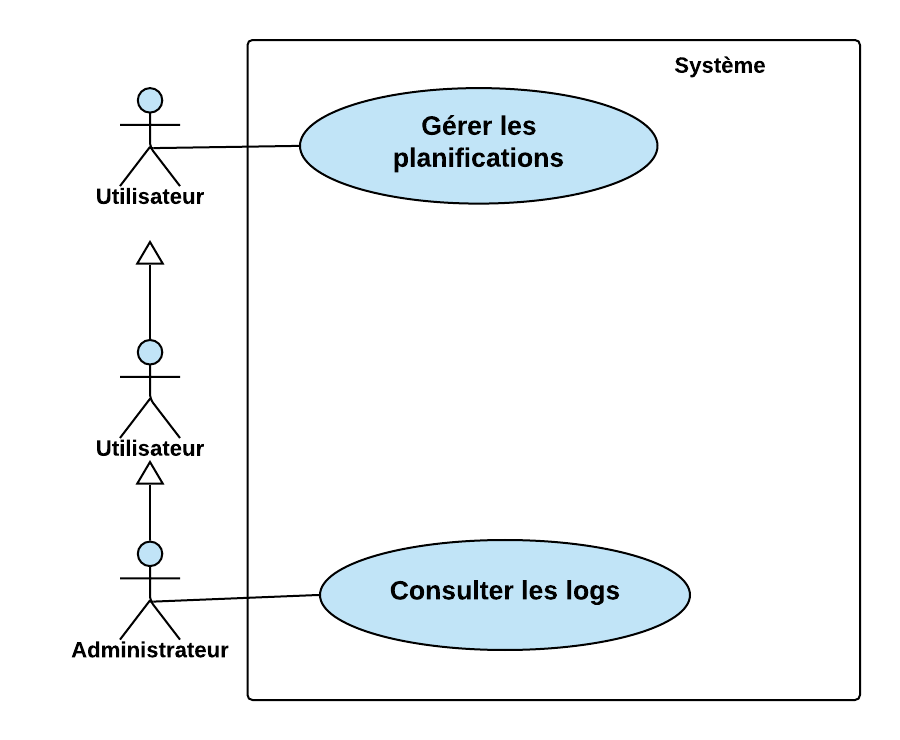
\includegraphics[scale=0.5]{sprint3.png}
	\caption{Diagramme de cas d'utilisation du sprint 3}
	\label{Diagramme de cas d'utilisation du sprint 3}
\end{figure} \\
Tel qu'en atteste la figure 5.1, ce sprint permet aux utilisateurs de gérer les planifications. Ainsi, il  permet à l'administrateur de consulter les logs.
\section{Gestion des planifications }
Cette section est dédiée à la gestion des planifications. Elle est constituée par le cas d'utilisation "Gérer les planifications".\\
 La réalisation de ce cette partie nécessite l'utilisation du planificateur de tâches Cron. Ce dernier 
 est un utilitaire linux  qui planifie l'exécution automatique d'une commande ou d'un script sur le serveur à une date et une heure spécifiées. Il est utile pour automatiser  des tâches répétitives.
 Dans notre cas, il va planifier le fonctionnement des machines virtuelles.
\subsection{Analyse}
Afin de mieux  détailler le fonctionnement et assimiler les cas d'utilisation de ce sprint, nous allons établir, dans cette section,  leurs raffinements en livrant une description sur les scénarios les plus importants.
\begin{itemize}
	\item \textbf{Raffinement du cas d'utilisation "Gérer les planifications"}
\end{itemize}
\begin{figure}[h]
	\centering
	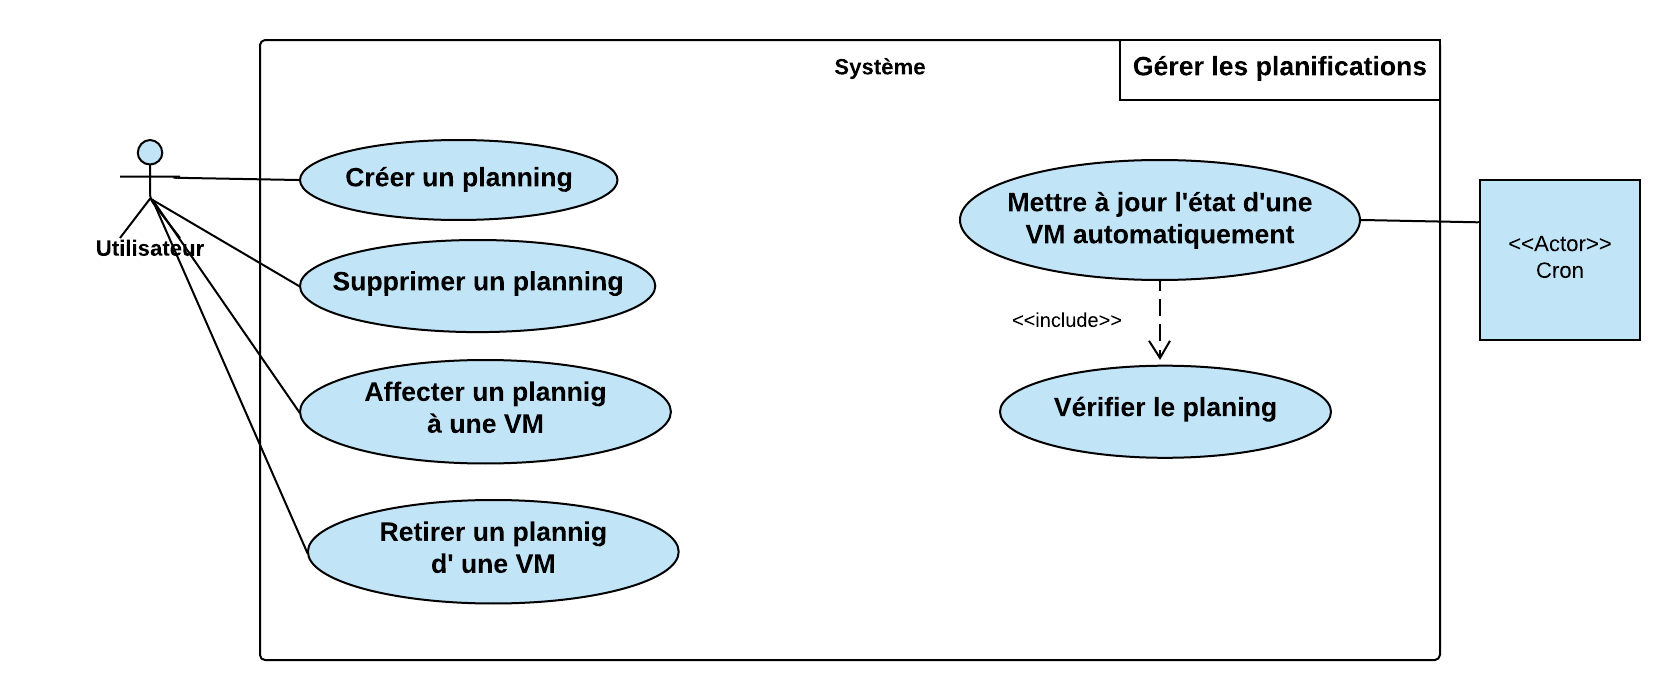
\includegraphics[ height=5.1cm, width=14cm]{Rgererplani.png}
	\caption{Raffinement du cas d'utilisation: Gérer les planifications}
	\label{Raffinement du cas d'utilisation: Gérer les planifications}
\end{figure} 
Comme le montre la figure 5.2, la création, suppression d'un planning et son  retrait  et affectation  à une VM sont tous des sous cas d'utilisation qui s'étendent de la gestion des planifications. En outre, la mise à jour automatique de l'état de la VM avec une vérification du planning affecté sont des cas d'utilisations assurés à travers notre second acteur qui est le Cron.

\subsubsection{Description textuelle du cas d'utilisation: "Supprimer un planning}

% Please add the following required packages to your document preamble:
% \usepackage{multirow}
\begin{table}[ht]
	\begin{tabular}{|l|l|}
		\hline
		\textbf{Acteur}                              & Utilisateur                                                                                                                \\ \hline
		\textbf{Description}                         & Supprimer un planning.                                                                                                     \\ \hline
		\textbf{Préconditions}                       & Utilisateur authentifié                                                                                                    \\ \hline
		\textbf{Post-conditions}                     & Planning supprimé.                                                                                                         \\ \hline
		\multirow{4}{*}{\textbf{Scénario principal}} & \begin{tabular}[c]{@{}l@{}}1. L'utilisateur sélectionne le planning et clique sur le bouton\\ de suppression.\end{tabular} \\ \cline{2-2} 
		& 2. Le système affiche une modale de confirmation.                                                                          \\ \cline{2-2} 
		& 3. L'utilisateur confirme son choix.                                                                                       \\ \cline{2-2} 
		& 4.  Le système supprime le planning correspondant.                                                                         \\ \hline
		\textbf{Scénario altérnatif}                 & 2.a L'utilisateur décide d'annuler son choix.                                                                              \\ \hline
	\end{tabular}

\caption{Description textuelle du << Supprimer un planning >> }
\label{Description textuelle du << Supprimer un planning >>}
\end{table}

\subsection{Conception}

Afin de décortiquer et détailler les cas d'utilisation précédemment cités, nous présentons dans ce qui suit les diagrammes de séquences des cas d'utilisation les plus importants
\subsubsection{Diagramme de séquence du cas d'utilisation: "Mettre à jour l'état d'une machine virtuelle automatiquement"}

\begin{figure}[H]
	\centering
	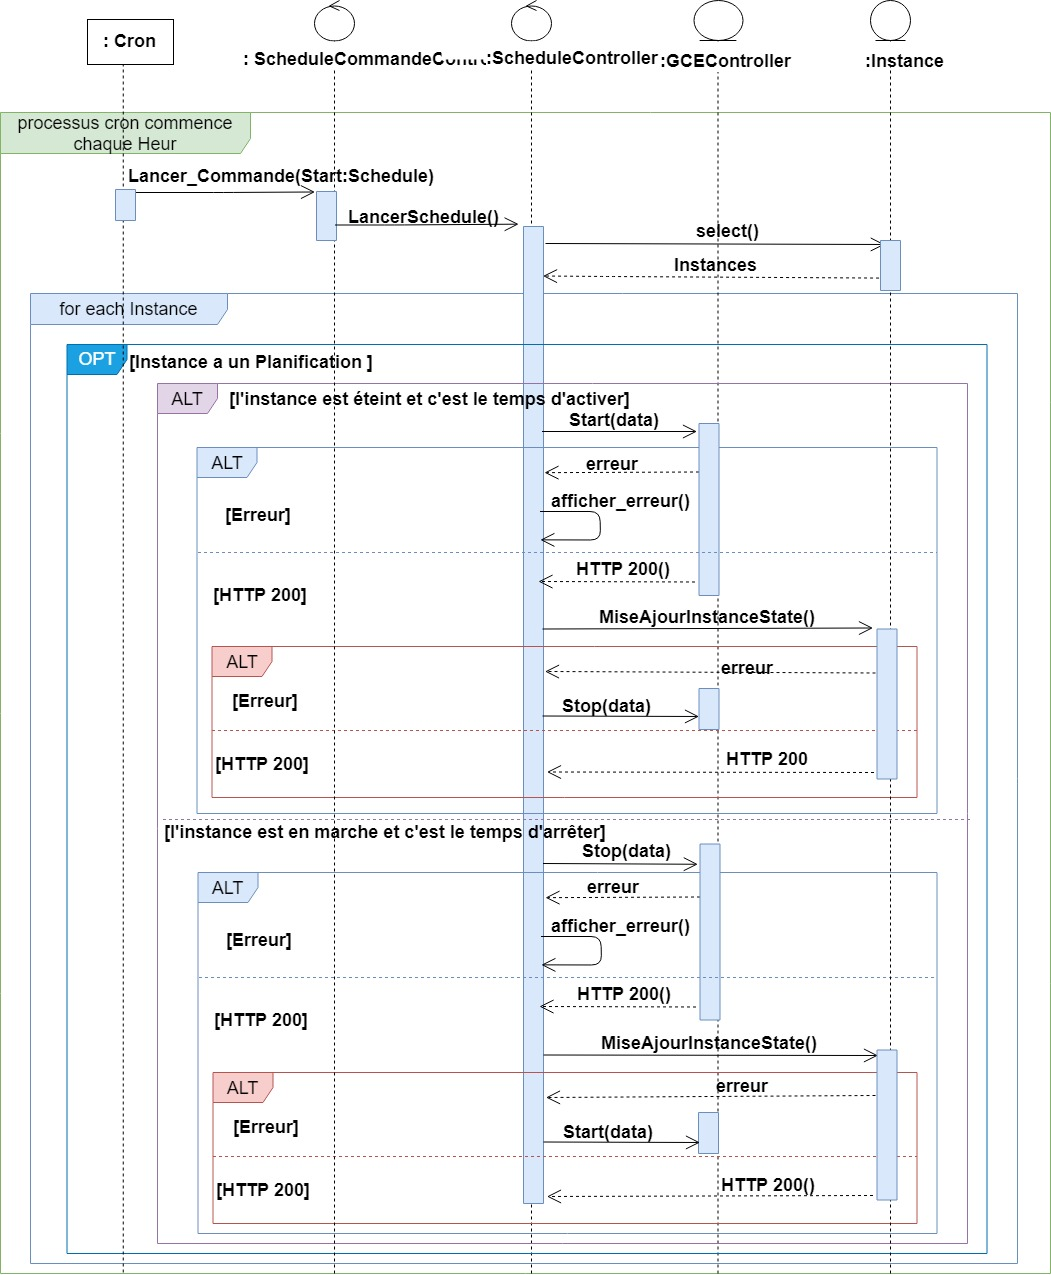
\includegraphics[ height=15cm, width=15cm]{schedule1.jpg}
	\caption{Diagramme de séquence: Mettre à jour l'état d'une machine virtuelle automatiquement}
	\label{Diagramme de séquence: Mettre à jour l'état d'une machine virtuelle automatiquement}
\end{figure}
Le diagramme de la figure 5.3 détaille la procédure relative à la mise  à jour automatique de l'état des VMs. Cette opération nécessite la mise en place de l'outil Cron de linux.
Chaque heure, cron demande la consommation de l'API responsable au fonctionnement  automatique des machines virtuelles. Au moment de l'exécution de cet API, le contrôleur des planifications récupère la liste des instances et pour chaque instance qui a un planning il vérifie  si elle est en état de repos et si son planning l'oblige pour qu'elle soit activée. Si c'est le cas,  le contrôleur émet une requête au Google Compute engine  pour l'activer et une  autre pour changer son état  dans la base de données. Dans le cas ou une erreur s'est produite au niveau de la mise à jour dans la base de données et pour en assurer la synchronisation le contrôleur annule l'opération en arrêtant la VM auprès de Google Compute Engine. 
Pareil pour l'arrêt automatique d'une machine mise en marche.
\subsubsection{Diagramme de séquence du cas d'utilisation: "Créer un planning"}

\begin{figure}[H]
	\centering
	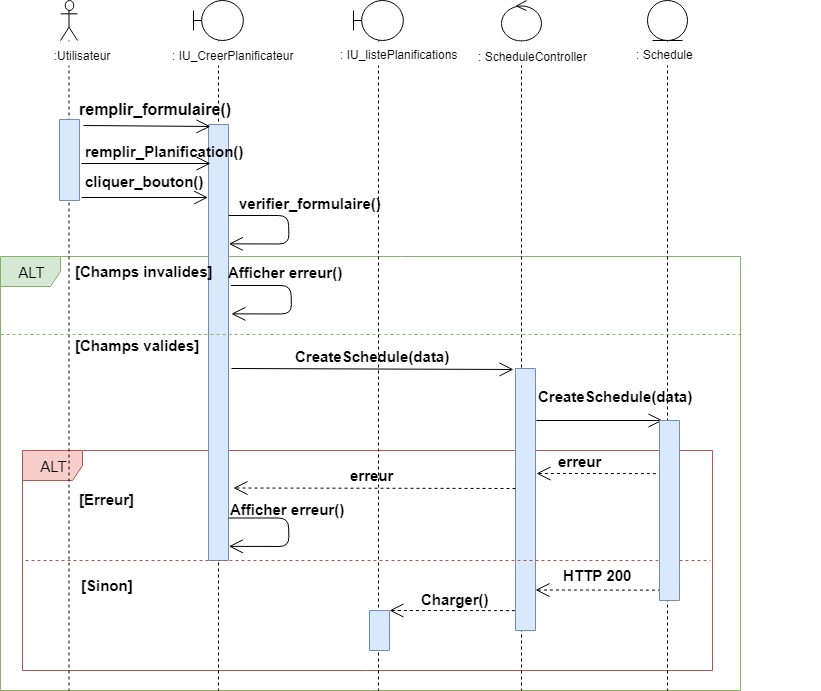
\includegraphics[scale=0.6]{createSchedule.png}
	\caption{Diagramme de séquence: Créer un planificateur}
	\label{Diagramme de séquence: Créer un planificateur}
\end{figure}
Le diagramme de la figure décrit l'opération de création d'un planning. Tout d'abord, l'utilisateur remplit le formulaire correspondant et choisit l'horaire du fonctionnement de  la machine virtuelle puis valide. Une fois validé, le contrôleur émet une requête de création d'un planning. Il retourne une requête de statut 200 si la création est effectuée avec succès et une erreur dans le cas contraire.
\section{Gestion des logs }
Cette section est dédiée à la gestion des logs. Elle est constituée par le cas d'utilisation "Consulter les logs".\\

\subsection{Analyse}
Dans ce qui suit, nous allons offrir une vue d'ensemble des fonctionnalités
relatives à la deuxième partie de ce sprint. 
\subsubsection{Description textuelle du cas d'utilisation: "Consulter les logs"}
% Please add the following required packages to your document preamble:
% \usepackage{multirow}
\begin{table}[H]
	\begin{tabular}{|l|l|}
		\hline
		\textbf{Acteur}                              & Administrateur.                                            \\ \hline
		\textbf{Description}                         & Afficher les logs.                                         \\ \hline
		\textbf{Préconditions}                       & Administrateur authentifié.                                \\ \hline
		\textbf{Post-conditions}                     & Liste des logs affichée.                                   \\ \hline
		\multirow{2}{*}{\textbf{Scénario principal}} & 1. L'administrateur demande la page des logs.              \\ \cline{2-2} 
		& 2. Le système charge les données et les retournes.         \\ \hline
		\textbf{Scénario altérnatif}                 & 2. Le système retourne une erreur du chargement de la page \\ \hline
	\end{tabular}

\caption{Description textuelle du << Consulter les logs >> }
\label{Description textuelle du << Consulter les logs >>}
\end{table}
\subsection{Conception}
Afin de décortiquer et détailler le cas d'utilisation précédemment cité, nous présentons dans ce qui suit sa conception à travers le diagramme de séquences objet.
\newline
\begin{figure}[H]
	\centering
	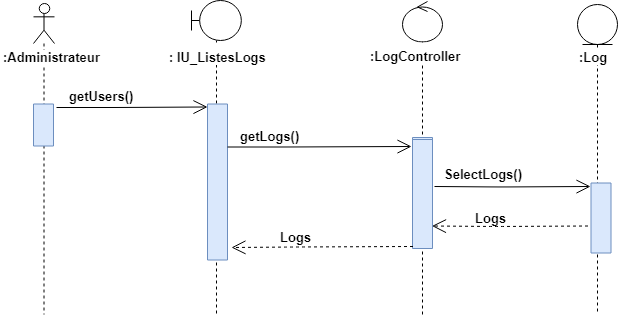
\includegraphics[scale=0.6]{listerLog.png}
	\caption{Diagramme de séquence: Consulter les logs}
	\label{Diagramme de séquence: Consulter les logs}
\end{figure}

Le diagramme de la figure décrit l'opération de sélection des logs. En effet, l'administrateur charge la pages contenant la  liste des logs. A ce moment, le contrôleur sélectionne  et retourne la liste des logs.
\section{Réalisation}
Après avoir achevé l'étape de la conception de ce sprint, en tenant compte des besoins fixés et des
choix conceptuels effectués  précédemment, nous consacrons cette section à la
description du travail réalisé.
\subsection{Interfaces}

\begin{figure}[H]
	\centering
	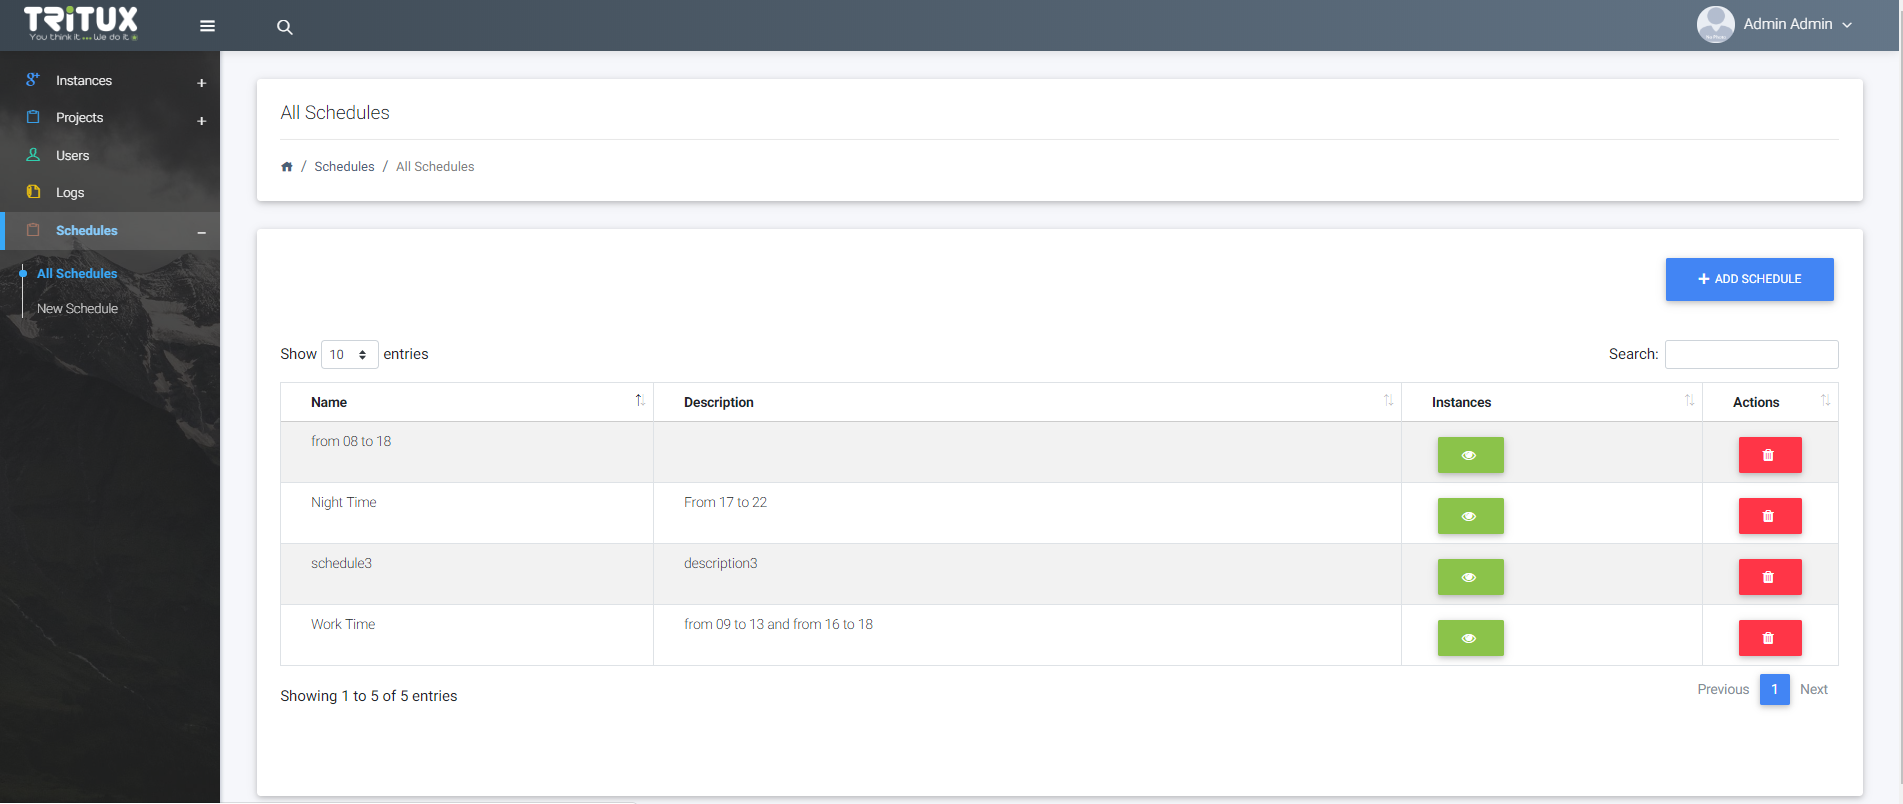
\includegraphics[scale=0.35]{schedules.PNG}
	\caption{Interface de gestion des planifications}
	\label{Interface de gestion des planifications}
\end{figure}
La figure 5.6 représente l'interface de gestion des planifications, grâce à laquelle l'utilisateur
pourra rechercher , supprimer  et  créer un nouveau planning comme le montre la figure 5.7 ci-dessous. 
\newline
\begin{figure}[H]
	\centering
	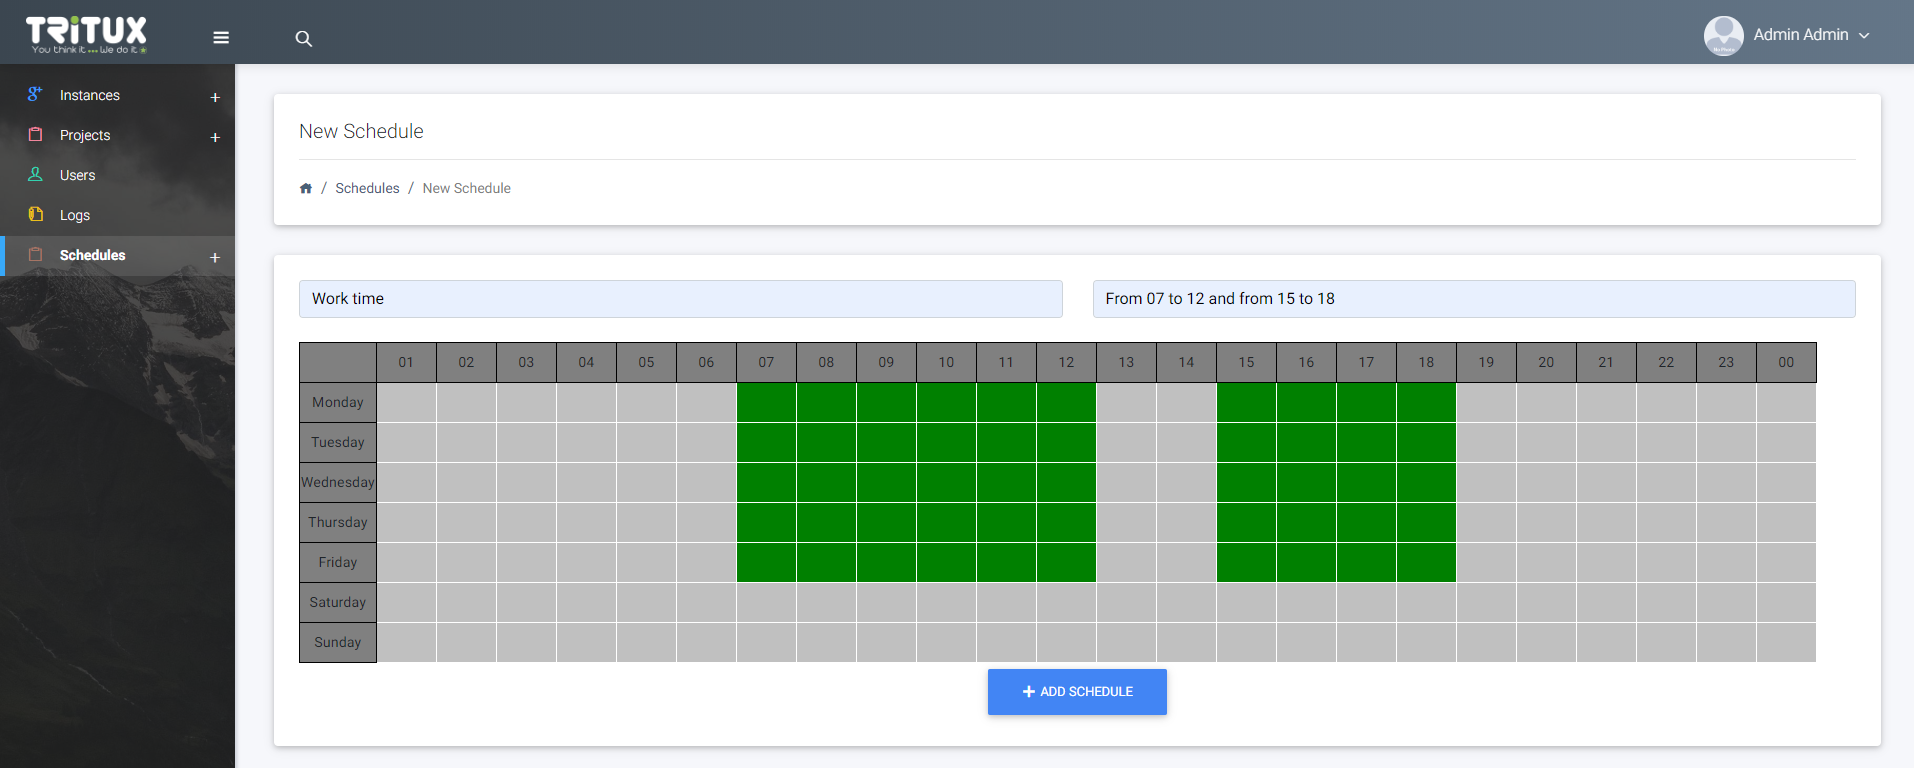
\includegraphics[scale=0.35]{creerschedule.PNG}
	\caption{Interface de création d'un planning}
	\label{Interface de création d'un planning}
\end{figure}
\begin{figure}[H]
	\centering
	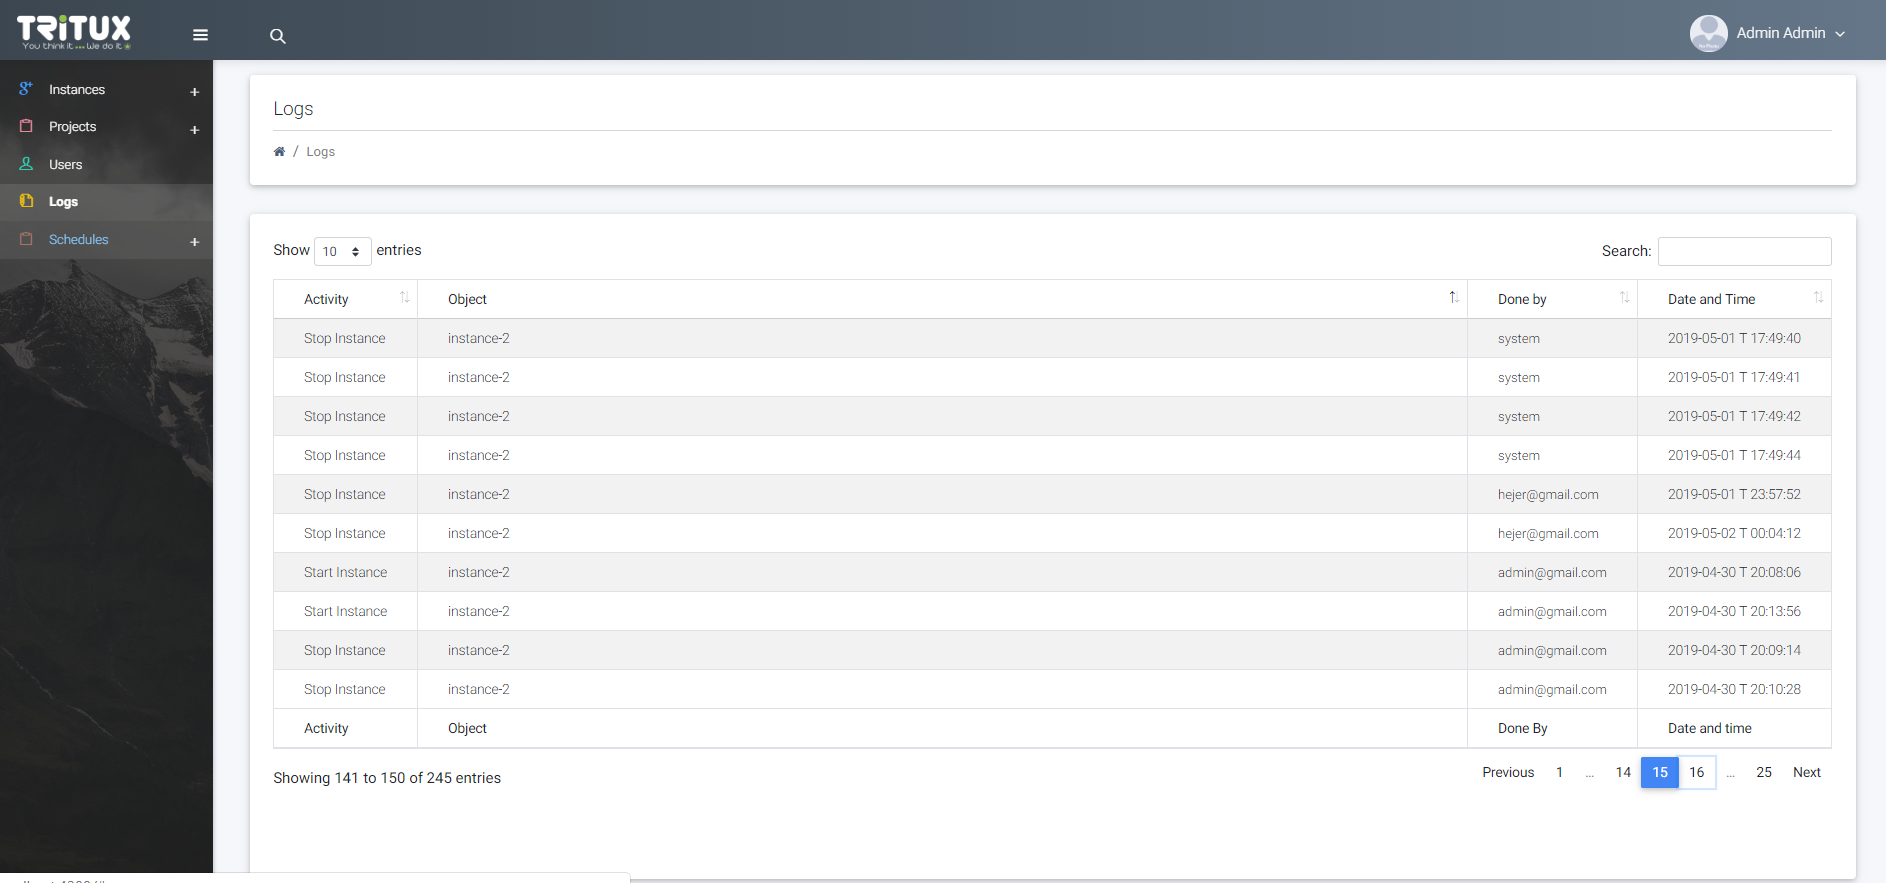
\includegraphics[scale=0.35]{logs.PNG}
	\caption{Interface de consultation des logs }
	\label{Interface de consultation des logs}
\end{figure}

La figure 5.8 ci dessus, représente l'interface grâce à laquelle l'administrateur peut accéder et consulter les logs de toutes les activités des utilisateurs dans l'application.
\section{Conclusion}
Nous clôturons ici la réalisation du dernier sprint de notre application. Nous avons pu réaliser les logs grâce
auquel l'administrateur aura une vue global des activités de ses collaborateurs ainsi que
la partie gestion des planifications pour automatiser le fonctionnement des machines virtuelles.